\documentclass{beamer}
\usepackage[polish]{babel}
\usepackage[utf8]{inputenc}
\usepackage[T1]{fontenc}
\usepackage{polski}
\usepackage{graphicx}
\usepackage{xcolor}
\usepackage{listings}
\usepackage{url}

\usepackage[backend=biber]{biblatex}
\addbibresource{bibliography.bib}

\lstset{
	literate=%
	{ą}{{\k{a}}}1
	{Ą}{{\k{A}}}1
	{ć}{{\'c}}1
	{Ć}{{\'{C}}}1
	{ę}{{\k{e}}}1
	{Ę}{{\k{E}}}1
	{ł}{{\l{}}}1
	{Ł}{{\L{}}}1
	{ń}{{\'n}}1
	{Ń}{{\'N}}1
	{ó}{{\'o}}1
	{Ó}{{\'O}}1
	{ś}{{\'s}}1
	{Ś}{{\'S}}1
	{ż}{{\.z}}1
	{Ż}{{\.Z}}1
	{ź}{{\'z}}1
	{Ź}{{\'Z}}1
}


\usetheme{Warsaw}
\usecolortheme{default}

\author{mgr~inż.~Rafał Kabaciński}
\title{Prezentacje w \LaTeX u}


\begin{document}


\begin{frame}
\titlepage
\end{frame}

\begin{frame}
	\tableofcontents
\end{frame}

\section{Podstawy}

\subsection{Wstęp}
	\begin{frame}[containsverbatim]
		\frametitle{Podstawy}
		
		\begin{block}{Klasa dokumentu}
			Prezentacje w środowisku \LaTeX\ tworzy się za pomocą klasy \emph{beamer}\\
			\verb|\documentclass{beamer}|
		\end{block}

		\begin{block}{Slajdy}
			Podstawową różnicą względem pracy w innych dokumentach jest konieczność definiowania kolejnych slajdów za pomocą otoczenia \emph{frame}:
			
			\begin{lstlisting}
\begin{frame}
	\frametitle{Podstawy}
\end{frame}
			\end{lstlisting}
			Użycie polecenia \verb|\frametitle{}| jest opcjonalne
		\end{block}
		
	\end{frame}

	\begin{frame}[containsverbatim]{Motywy}
		Podstawowy styl prezentacji definiuje się za pomocą polecenia:
		\begin{center}
			\verb|\usetheme{Warsaw}|
		\end{center}
		Natomiast zestaw kolorów za pomocą polecenia:
		\begin{center}
			\verb|\usecolortheme{default}|
		\end{center}
		Podstawowy zestaw stylów i zestawów kolorów sprawdzić można na stronie: \url{https://hartwork.org/beamer-theme-matrix/}
		\begin{center}
		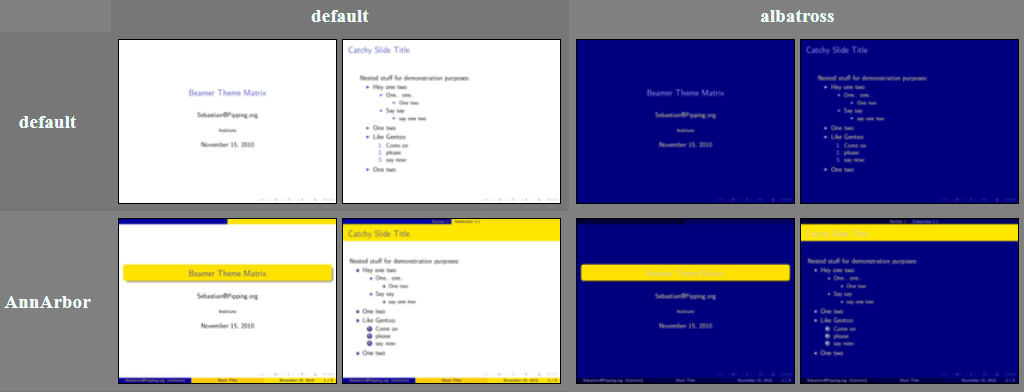
\includegraphics[width=0.8\textwidth]{Ilustracje/Thems}
		\end{center}

	\end{frame}
	
	\subsection{Bloki}
	\begin{frame}[fragile]{Bloki}
		
	Fragmenty tekstu na prezentacjach można zamykać w blokach z własnymi tytułami:

	\begin{columns}
		\column{0.66\textwidth}
		
		\begin{lstlisting}
\begin{block}{Zwykły blok}
	Treść
\end{block}
		\end{lstlisting}
		
		\begin{lstlisting}
\begin{alertblock}{Ważny blok}
	Treść
\end{alertblock}
		\end{lstlisting}
		
	\column{0.33\textwidth}

	\begin{block}{Zwykły blok}
	Treść
	\end{block}
	\vspace{5mm}
	\begin{alertblock}{Ważny blok}
	Treść
	\end{alertblock}

	\end{columns}
	\end{frame}

\section{Treść prezentacji}
\subsection{Podział logiczny}
\begin{frame}[fragile]{Podział logiczny}
	\begin{block}{Spis treści}
		Spis treści wstawia się za pomocą polecenia:
		\begin{center}
			\verb|\tableofcontents|
		\end{center}

	\end{block}
	\begin{block}{Podział dokumentu}
		Najwyższym stopniem podziału prezentacji są sekcje.
		Poleceń podziału prezentacji powinno używać się pomiędzy otoczeniami \emph{frame}
	\end{block}
\end{frame}

\subsection{Podział na kolumny}
\begin{frame}[fragile]{Podział na kolumny}
	Slajd można podzielić na dwie kolumny za pomocą polecenia \emph{columns}
	\begin{block}{Przykład}
		\begin{lstlisting}
\begin{columns}
	\column{0.66\textwidth}
	Szersza kolumna
	\column{0.33\textwidth}
	Węższa kolumna
\end{columns}
		\end{lstlisting}
	\end{block}
	\begin{columns}
		\column{0.66\textwidth}
		Szersza kolumna
		\column{0.33\textwidth}
		Węższa kolumna
	\end{columns}
\end{frame}

\subsection{Kod źródłowy}
\begin{frame}[fragile]{Kod źródłowy}
	Na slajdach można wstawiać kod źródłowy za pomocą poleceń \emph{verb} jak i otoczeń \emph{lstlisting}. Konieczne jest jednak oznaczenie danego slajdu za pomocą argumentu opcjonalnego:
	
	\begin{block}{Przykład}
	\verb|\begin{frame}[fragile]|\\
	\verb|	\begin{lstlisting}|\\
	\verb|		Kod źródłowy|\\
	\verb|	\end{lstlisting}|\\
	\verb|\end{frame}|
	\end{block}
\end{frame}

\end{document}